% !TEX encoding = UTF-8 Unicode
\documentclass{01_preamble/report}
% big font for sections
%\usepackage{sectsty}
%\sectionfont{\LARGE}

\usepackage{graphicx}
\usepackage{wrapfig}
\usepackage[labelfont={bf,sf}]{caption}
\usepackage{subcaption}
\usepackage{listings}
\usepackage{hyperref}
\usepackage{blindtext}
\usepackage{amssymb}
\usepackage{amsmath}
\usepackage{bm}
\usepackage{amsmath}
% SET TITLE SECTION INFORMATION 
\title{Political Economics - Lecture notes}

\author[1]{Kristian Urup Olesen Larsen}
\affil[1]{Department of Economics, University of Copenhagen} 

\dates{\today}
	
% REFERENCES SETUP
\usepackage[round, authoryear, sort&compress]{natbib}
\bibliographystyle{unsrtnat}

% SET TITLES OF CONTENTS AND REFERENCES
\addto\captionsenglish{% Replace "english" with the language you use
  \renewcommand{\contentsname}%
    {Table of Contents}%
}
\renewcommand{\refname}{References}
    
\numberwithin{equation}{section}

\begin{document}
\maketitle
\vskip24pt
\begin{abstract}
    These are notes for the course "Auctions, theory and practice". Some of the content is probably wrong or poorly explained.
\end{abstract}
\vskip24pt
% COMMENT NEXT LINE TO REMOVE TABLE OF CONTENTS
\tableofcontents\vskip48pt
\dropcap{T}his is my lecture notes for the course \emph{political economics} taught at the Department of Economics at the University of Copenhagen. I've written these notes as a student, and as such some of the material might be wrong. If you find any mistakes please create an issue on github and i will correct it. 

%=================
\section*{Part 1}
\section{Lecture 1 - Introduction}\label{seq: lecture1}
This course is about political \textit{economics}, i.e. studying how political systems affect outcomes. The course is not about political \textit{economy} which is the old-school Marx/Smith economics. Also this course is not about international political economics, which is concerned with the functions of international organizations and regimes.

What we want to do is to understand and explain differences and similarities in economic policy across time, varying political regimes and geography. 

\subsection{Political preferences and majority voting (the median voter model)}
The median voter model is a workhorse of the field, and we will use it throughout the course. In it we assume that policy is determined by simple majority voting. 

Consider a society with $N$ agents, who each have quasi-linear utility $w^i$ of consumption $c^i$ and leisure $x^i$ such that 
\begin{equation}
  w^i = c^i + V(x^i), \quad V'> 0, V''<0
\end{equation}
Individuals are all taxed by some fixed share $(1-q)$ of their income $I^i$, and in return receive a fixed transfer $f$, meaning we can write an individuals budget constraint as 
\begin{equation}
  c^i = (1-q)I^i + f
\end{equation}
Normalizing the wage to $1$ across all individuals we can simply read $I^i$ as the labor supply. A simple way to introduce agent heterogeneity with singular wages is to let the available time for labor be heterogeneous, so instead of having $1=I^i + x^i$, i.e. total time is fully spent either on labor or leisure we induce some variation in the total time available $\alpha^i$ 
\begin{equation}
  1- \alpha^i = I^i + x^i
\end{equation}
We denote the mean of $\alpha^i$'s in the population by $\alpha$ and the median by $\alpha^m$. 

\subsubsection{Agent maximization problem}
From the perspective of a single agent the tax rate $q$ is fixed, so they simply solve 
\begin{equation}
  \begin{split}
    & \max_{I^i} c^i + V(x^i) \\
    & \quad \text{s.t. } c^i = (1-q)I^i + f \\ 
    & \quad \text{and } 1-\alpha^i = I^i + x^i
  \end{split}
\end{equation}
Inserting the constraints and taking the derivative w.r.t $I^i$ we get a first order condition of  
\begin{equation}
  (1-q) = V'(1-\alpha^i - I^i)
\end{equation}
That is agents choose their labor supply to balance the net income gain from supplying an additional unit of labor with the marginal increase in utility from having one more unit of leisure. Isolating the labor supply we find that 
\begin{equation}
  \begin{split}
  I^{i*} &= 1- \alpha^i -V'^{-1}(1-q) \\ 
  &= 1- \alpha^i -V'^{-1}(1-q) - \alpha + \alpha \\ 
  &= L(q) - (\alpha^i - \alpha)
  \end{split}
\end{equation}
where $L(q) \equiv 1- \alpha - V'^{-1}(1-q)$ can be shown to be the average labor supply in the population (in equilibrium). To see this notice 
\begin{equation}
  I \equiv \frac{1}{N} \sum_{i=1}^N I^i = \sum_{i=1}^N \left[ L(q) - (\alpha^i - \alpha) \right] = L(q)
\end{equation}

\subsubsection{Indirect utility}
Let us assume that the government runs a balanced budget, meaning the transfer individual must be equal to the taxes raised from the average individual, that is 
\begin{equation}
  f = qL(q)
\end{equation}
The indirect utility of an agent is then utility which is achieved by optimally setting the labor supply given $q$, put intuitively: now we know how agents behave for any given $q$ and we know how the government sets $q$, so we can write the indirect utility each agent gets for any choice of $q$: 
\begin{equation} \label{eq: indirectutility}
  \begin{split}
    W(q, \alpha^i) &= c^i + V(x^i) \\ 
    &= (1-q)I^i + f + V(1-\alpha^i - I^i) \\ 
    &= (1-q)\underbrace{\left[L(q) - (\alpha^i - \alpha) \right]}_{\text{optimal $I^i$ given } q} + \underbrace{qL(q)}_{\text{GBC}} + \underbrace{V(1 - L(q) - \alpha)}_{\text{insert } I^{i*}}
  \end{split}
\end{equation}
This expression shows us how each agents utility will be in optimum given some $q$ and some preferences $V(\cdot)$. Now in an election individuals recognize that they should not simply vote for the $q$ that optimizes their utility given static labor supply, instead they should vote for the $q$ that yields the highest utility after making changes to ones labor supply. The policy which satisfies 
\begin{equation}
  q(\alpha^i) = \text{arg max}_q W(q, \alpha^i)
\end{equation}
is called the \textit{bliss point} of agent $i$, as this is the ideal choice of policy for this agent. In general this will depend on $\alpha^i$ (imagine someone with $\alpha^i=1$, they have no change of earning labor income and might as well prefer a very high $q$). 

\subsection{Majority rule voting}
Now knowing how each individual would prefer the tax rate to be set we need a way to aggregate individual wishes into a single global tax rate which applies to everyone. One option is to implement pure majority voting, that is a system with
\begin{enumerate}
\item Direct democracy, whatever citizens vote for will be the outcome. 
\item Sincere voting, agents vote for the policy that is their bliss point (no strategic voting).
\item Open agenda voting, for all possible pairs $q_1, q_2$ citizens vote for their prefered option untill all combinations have been tried against each other.   
\end{enumerate}

This naturally is not exactly how democracies work, but it serves as a useful framework for modelling the dynamics at play in voting systems. 

\paragraph{Arrows imposibility theorem}
Arrows impossibility theorem states that there is three or more choices for voters to choose from, no ranked voting system (i.e. majority voting) can convert individual votes into a community choice which fulfils 

\begin{enumerate}
  \item Unrestricted domain: all preferences are allowable, there is no requirement for consistency in policy preferences. 
  \item non-dictatorship: Voters actually matter for the final choice (it is not simply a benevolent social planner who chooses the best option).
  \item Pareto efficency: there is no pareto improvements to be made. 
  \item Independence of irrelevant alternatives: if some given policy is prefered, it should still be prefered in an election with only a subset (including $q$) of the options available.
\end{enumerate}

\paragraph{Condorcet winners} Without any restriction on the election it is possible to have condorcet cycles, which is essentially a set of preferences that is cyclic over some set of alternatives, so $a>b$, $b>c$ and $c>a$ would constitute a condorcet cycle.

A \textit{condorcet winner} on the other hand is a policy $q^*$ which can beat any alternative $q$ in a pairwise vote of $(q^*, q)$. It can be shown that under majority voting, with $q\in\mathbb{R}$ a condorcet winner exists if voters preferences are single peaked, that is if
\begin{equation}\label{eq: singlepeak}
  q'' \leq q' \leq q(\alpha^i) \text{ or } q'' \geq q' \geq q(\alpha^i) \Rightarrow W(q'', \alpha^i) \leq W(q', \alpha^i)
\end{equation}
This equation essentially states that for each individual the indirect utility is monotonically decreasing on both sides of $q(\alpha^i)$. This assumption is strong - it is the indirect utility that must behave nicely, not the direct utility. 
The condorcet winner will furthermore be equal to the median voters prefered policy $q^m$. To see this see that any $q'<q^m$ will have support from less than half the population and so $q^m$ would win in a pairwise vote. This argument is then identical for $q'>q^m$.
\\ \\ 
Returning to the indirect utility derived in (\ref{eq: indirectutility}) we can show that this does not satisfy single peakedness as defined in (\ref{eq: singlepeak}) for sufficiently large $\frac{\partial^2}{\partial q \partial q} L(q)$. To see this note that a positive second derivative corresponds to an graph that is convex implying at least no equilibrium, or of this property is only piecewise that there are multiple equilibria. The second derivative is straight forward to derive as 
\begin{equation}
\frac{\partial^2}{\partial q \partial q} = (1+V'(\cdot))L''(q) + V''(\cdot)L'(q)^2  
\end{equation}
By assumption $V'>0$ and $V''<0$ so we loose single peakedness when the first term is larger than the second, or with a bit of rearranging: 
\begin{equation}
  L''(q) > \frac{V''(\cdot)}{1 + V'(\cdot)} L'(q)^2
\end{equation}

\paragraph{Single crossing preferences} An alternative to the single peaked preferences assumption is to assume the \emph{single crossing} property. This is different form single peakedness as it not only involves assumptions about the shape of individual agents utility functions, but makes assumptions about the distribution of voter types, specifically assume $\alpha^i \in \upsilon$ where $\upsilon$ is some set of voters. The single crossing property is then that if

\begin{equation}\label{eq: singlecrossing}
  \begin{split}
&  (\alpha^i < \alpha^{i'} \text{ and } q > q') \text{ or } (\alpha^i > \alpha^{i'} \text{ and } q<q') \\ 
&  \text{then } W(q, \alpha^i) \geq W(q', \alpha^i) \Rightarrow 
  W(q, \alpha^{i'}) \geq W(q', \alpha^{i'}) 
  \end{split}
\end{equation}
That is, if we consider two agents and two possible policies such that a) the "stronger" agent prefers the highest tax or b) the "weaker" agent prefers the lower tax, then we can infer that a) the "weaker" agent also prefers the highest tax or b) The "stronger" agent also prefers the lower tax. In other words relatively more extreme individuals prefer policies that are also more extreme. Notice how this is an assumption on the distribution of preferences across $\alpha^i$'s while single-peakedness was an assumption about the individual preferences for a given $\alpha^i$. When individuals satisfy the single crossing asusmption the median policy $q^m$ will be the condorcet winner and equilibrium policy. 

\paragraph{Proof that single crossing leads to $q^m$:} Think of the median type $\alpha^m$ who naturally has prefered policy $q^m$. Any $q<q^m$ will be dismissed by $\alpha^m$ and any agents with $\alpha^i > \alpha^m$ giving a majority to $q^m$. Likewise for any $q>q^m$.    

We can show that the expression in (\ref{eq: indirectutility}) does satisfy the single crossing property in (\ref{eq: singlecrossing}). To see this notice that when adding and subtracting $(1-q)\alpha^i$ to (\ref{eq: indirectutility}) we get 
\begin{equation} \label{eq: indirectrewriten}
  \begin{split}
    W(q, \alpha^{i'}) &= L(q) - V(1-L(q)-\alpha) -(1-q)(\alpha^{i'} - \alpha^i) - (1-q)(\alpha^i - \alpha) \\ 
  &= W(q, \alpha^i) - (1-q)(\alpha^{i'} - \alpha^i)    
  \end{split}
\end{equation}
So consider a case where individual $\alpha^{i'}$ prefers $q$ to $q'$, i.e.
\begin{equation}
  W(q, \alpha^{i'}) \geq W(q', \alpha^{i'})
\end{equation}
From the rewrite in (\ref{eq: indirectrewriten}) this directly implies 
\begin{equation}
  W(q, \alpha^{i}) - (1-q)(\alpha^{i'}- \alpha^i) \geq 
  W(q', \alpha^{i}) - (1-q')(\alpha^{i'}- \alpha^i)
\end{equation}
Rearanging we then have 
\begin{equation}
  W(q, \alpha^i) \geq W(q', \alpha^i) - (q'-q)(\alpha^{i'} - \alpha^i)
\end{equation}
Now notice that if $(q'-q)(\alpha^{i'} - \alpha^i) \geq 0$ we have shown that $W(q, \alpha^{i'}) \geq W(q', \alpha^{i'})$ implies $W(q, \alpha^i) \geq W(q', \alpha^i)$. Since $(q'-q)(\alpha^{i'} - \alpha^i) \geq 0$ is logically identical to the requirements posed in the single crossing definition, and the implication is exactly what the single crossing property entails, we have shown that our model does have the single crossing property. 

\subsection{Reflections on the median voter theorem}
Everything above relies on the policy being single dimensional, which is probably a poor fit for the real world. However we could consider this single dimension to not be as conrete as a tax rate, but rather a "left-right" leaning, in which case one could argue for some kind of single-dimensionality. Without a single dimensional policy, it is however not generally possible to find a condorcet winner. 

\section{Electoral competition I}
In this lecture we will begin studying a model of electoral competition, that is a model for how politicians propose platforms in the competition to be elected. We consider two party competition where there is one policy objective (e.g. the size of the public sector) and politicians are opportunistic i.e. they have only one goal, which is getting elected. Politicians must commit to a proposal before the election and must provide this policy after being elected (this doesn't matter to much when their only goal is getting elected). 

\paragraph{Model setup} Consider a continuum of citizens with quasi-linear utility from consumption $c_i$ and a public good $g$ so 
\begin{equation} \label{eq: downsutility}
    w^i = c^i + H(g)
\end{equation}
Individuals are taxed and accordingly have a budget constraint of  
\begin{equation}
    c^i=(1-\tau)y^i
\end{equation}
Here $y^i$ is distributed according to $F(\cdot)$ so that $E[y^i]=y$, the median income is $y^m$ so $F(y^m)=1/2$ and we assume that $y^m < y$ implying a right skewed distribution of income. 

The government earns taxes $\tau$ and uses these to provide the public good $g$ so 
\begin{equation}
    g = \int \tau y^i f(y^i) \ dy^i = \tau y
\end{equation} 
The \textit{indirect utility} can then be found by inserting the governments budget constraint in (\ref{eq: downsutility}):
\begin{equation} \label{eq: indirectutilityDowns}
    \begin{split}
    W^i(g) &= \left(1 - \frac{g}{y}\right)y^i + H(g) \\ 
    &= (y-g)\frac{y_i}{y} + H(g)
    \end{split}
\end{equation}
This equation shows the central tradeoff in the model, namely that individuals gain utility from increasing $g$ but then face paying a higher tax reflected in the fact that higher $g$ decreases the utility from private consumption. The loss of private consumption is more costly for individuals with a higher income.

\paragraph{Prefered policy} We can solve for an agents preferred policy by maximizing the indirect utility w.r.t. $g$, 
\begin{equation}
    \frac{\partial W^i}{\partial g} = -\frac{y^i}{y} + H_g(g) \qquad (=0)
\end{equation}
where $H_g$ is the derivative of $H$ w.r.t. $g$. Solving for $g$ shows that the individuals optimal policy level is 
\begin{equation} \label{eq: downsequi}
    g^i = H_g^{-1}\left( \frac{y^i}{y} \right)
\end{equation}
By assumption $H$ is strictly concave and since the first term in $W^i$ is linear, we can infer that this too is strictly concave. This in turn tells us that \textit{preferences are single peaked} in this model. By this logic we can also infer that $H_g^{-1}$ is decreasing in $y^i$. So higher income individuals prefer less of the public good, intuitively this is because high income implies a large marginal cost of increased taxes, while the marginal benefit of $g$ is identical across all individuals. 

\subsection{A benchmark for election performance}
Before we study how elections affect the choice of $g$, let's first consider what level a benevolent social planner (i.e. a good dictator) would choose. The utilitarian welfare function is simply 
\begin{equation}
    SWF^U = \int_{y^i} W^i(g)f(y^i) \d y^i
\end{equation}
i.e. the aggregated indirect utility over all individuals. Inserting in this equation we can simplify the expression quite a bit 
\begin{equation}
    \begin{split}
        SWF^U &= \int_{y^i} \underbrace{\left( (y-g)\frac{y^i}{y} + H(g)  \right)}_{W^i(g)}f(y^i) \ dy^i \\ 
        &= W(g)
    \end{split}
\end{equation}   
where $W(g)$ is the average indirect utility, or equivalently the indirect utility of the individual with $y^i=y$. The social planner accordingly would provide a level of $g$ equal to 
\begin{equation}
    g^* = H_g^{-1}(1)
\end{equation}
which is simply (\ref{eq: downsequi}) evaluated for the average voter (we get the 1 from dividing $y/y$).

\subsection{Downsian electoral competition}
Now instead of a social planner let us consider a situation where there is held an election for the political position to choose $g$. There are two parties $P=A,B$ and the probability that candidate $P$ wins the election we denote $p_P$. Candidates receive an "ego-rent" $R$ from holding office and get 0 if they loose, consequentially they seek to maximize $p_P \cdot R$. The share of votes each candidate receive we denote $\pi_P$, and using this we can write $p_A$ and $p_B$ as 
\begin{equation}
    \begin{split}
        p_A &= Pr[\pi_A > 1/2 | g_A, g_B] \\ 
        p_B &= 1-p_A
    \end{split}
\end{equation}
Once again we assume that voters vote sincerely. The proposals $g_A, g_B$ are announced before the election. 

\paragraph{Simple example} Let us first assume that all voters have the same income so $y^i=y$ and $W^i(g)=W(g)$ for all $i$. In this case 
\begin{equation}
 p_A =  
    \begin{cases}
       1, \qquad \text{if } W(g_A) > W(g_B) \\ 
       1/2, \quad \text{if } W(g_A) = W(g_B) \\
       0, \qquad \text{if } W(g_A) < W(g_B) 
    \end{cases}
\end{equation}
and of course $p_B=1-p_A$. In this case there is an unique Nash equilibrium where $g_A=g_B=g^*$. To see this notice that $g^*$ maximizes $W(g)$ by definition. Any deviation from this level by either candidate will therefore immediately set $p_P=0$ which gives the politician utility $0<\frac{1}{2}R$. In this case we can thus say that political competition induces politicians to propose good policies.

\paragraph{Adding variation in $\bm{y^i}$} Now let us assume that $y^i\sim F(y^i)$. Because voters preferences are single peaked we know from the median voter theorem that the median voters preferred policy will be a condorcet winner and have majority support. Therefore we now have
\begin{equation}
    p_A =  
       \begin{cases}
          1, \qquad \text{if } W^m(g_A) > W^m(g_B) \\ 
          1/2, \quad \text{if } W^m(g_A) = W^m(g_B) \\
          0, \qquad \text{if } W^m(g_A) < W^m(g_B) 
       \end{cases}
\end{equation}
Where $W^m$ is the indirect utility of the median voter. Following a similar argumentation as before the Nash equilibrium will therefore be for both politicians to propose $g_A = g_B = g^m$.

Now because of the skewness in the income distribution we have that $y^m/y<1$. Because $H_g^{-1}$ is decreasing this implies
\begin{equation}
    g^m = H_g^{-1}(y^m/y) > H_g^{-1}(1) = g^*
\end{equation}
which is to say with varying income politicians propose a higher level of $g$ than what is optimal. This is because every voters vote counts equally so politicians can disregard the fact that taxation is extremely costly to those with the highest income. The social planner on the other hand takes this into account. This model gives us a testable prediction, which is that a more skewed income distribution should produce larger public sectors. 

\paragraph{Voters vs. tax payers} Notice that politicians only care about the part of their population that is eligible to vote. So the relevant measure of $y^m$ should be calculated only within the voters. Notice that $y$ should be calculated within the full population as this enters the equations through the taxes, which we assume you must pay regardless of your voting status. 
If some of the population is not eligible to vote we have to take this into account. One way to test the consequences of a more skewed distribution is thus to consider changes to voter eligibility laws which allow poor people to vote. These purely affect $y^m$ while leaving $y$ unaffected. 

\subsection{Beyond the median, \cite{gerber_beyond_2004}}
The paper by \citeauthor{gerber_beyond_2004} gather data from 2.8 million individuals votes from Los Angeles county in the 1992 general election. The data contains information on individuals voters choices in elections on all levels and includes votes on concrete policy proposals. From these data they estimate a county-level distribution of voters policy preferences. This lets the authors infer the policy position of the median candidate in each district. 

The authors also measure politicians behavior in whatever chamber they are elected to. This allows them to estimate the position on the liberal-conservative axis of each politician (both elected in LA and not). 
\\ \\
With these informations the authors can ask whether the position of the median voter in the local district affects the position of politicians. According to the median voter theorem politicians should vote in accordance with their local median voter, but it is obvious that peer and party effects can be competing explanations. The authors regress the preferred policy of LA politicians on the local median voters position as well as the median position of the own-party delegation in whatever chamber the politician has been elected to. 
\\ \\ 
The authors also investigate the role of district heterogeneity by interacting the median voters preferred policy with the variance of voters positions within the district. 
\\ \\ 
The authors find a significant role of median voters preferences \textit{in districts with homogeneous voters}. In heterogeneous districts this effect doesn't seem to exist to nearly the same degree. The authors also find evidence from peer effects in political stances.

\section{Electoral competition II}
So far we've studied a version of the downsian model with full policy convergence which implies that the median voter theorem also applies to representative voting democracies. This has revealed an important mechanism which forces politicians to run on popular platforms, often called the \textit{affect} mechanism.
\\ \\ 
There are however good arguments against the downsian model. First of it's conclusions are mainly based on the discontinuity in probability of winning, disregarding any uncertainty about voters preferences. Additionally the model must obviously be incomplete, as other things than the preferences of the median voter surely must matter to some degree. 

\subsection{Probabilistic voting} 
We will now relax the assumption about perfect information about voters preferences. We do this by introducing a candidate specific trait (e.g. ideology) which voters have preferences about. Importantly we assume uncertainty on the distribution of voter preferences with regards to this dimension. 
\\ \\ 
We depart from exactly the same point as last time, so the modelling framework is identical. This time however we assume there are three population groups $J=R,M,P$. Within groups income is identical at $y^J$ and they therefore also have the same indirect utility function $W^J$. Each groups share of the total population is given by $\alpha^J=\alpha^R,\alpha^M, \alpha^P$, and we assume that $y^R>y^M>y^P$. The average income in the population is 
\begin{equation}
    y = \sum_J \alpha^J y^J
\end{equation}
The voters care about $g$ as well as ideology, captured by the two bias-parameters $\sigma^{iJ}$ and $\delta$ which capture bias in direction of candidate $B$ (w.l.o.g.). Thus voters in group $J$ prefer candidate $A$ iff 
\begin{equation} \label{eq: probabilityChoice}
    W^J(g_A) > W^J(g_B) + \sigma^{iJ} + \delta
\end{equation}
We assume that
\begin{equation}
    \sigma^{iJ} \sim U\left(\frac{-1}{2\phi^J},\frac{1}{2\phi^J} \right) \qquad 
   \delta \sim U\left(\frac{-1}{2\psi},\frac{1}{2\psi} \right)
\end{equation}
The bounds of the distributions are simply chosen to simplify calculations. The important parts are that a) bias parameters are equally likely to be positive or negative, so the bias can be both in favor and disfavor of candidate $B$ with equal probability. And b) a higher $\phi^J$ (or $\psi$) implies more moderate voters, in the sense their votes are less likely to be tilted by ideology. 

In this setup $\sigma^{iJ}$ measures varying degrees of ideological focus within each income group, while $\delta$ measures an aggregate bias across the whole population, e.g. from scandals, campaigning etc.

\paragraph{Probability of winning} The parties want to maximize the probability of winning. Notice first that within each group $J$ we can identify the swing voter by the $\sigma^{iJ}$ that solves the equation in (\ref{eq: probabilityChoice}) with equality, that is the swing voter will have 
\begin{equation}
    \sigma^J \equiv  W^J(g_A) - W^J(g_B)  - \delta
\end{equation}
As all voters in $J$ with $\sigma^{iJ} < \sigma^J$ will vote for candidate $A$. Since $\sigma^{iJ}$ is uniformly distributed we can calculate the share that votes for candidate $A$ as\footnote{Recall in the uniform distribution on $[a,b]$, $F(x)=\frac{x-a}{b-a}$} 
\begin{equation}
    \begin{split}
        F^J(\sigma^J) &= \frac{\sigma^J + (2\phi^J)^{-1}}{2(2\phi^J)^{-1}} \\ 
        &= \phi^J\left(\sigma^J + \frac{1}{2\phi^J} \right) \\ 
        &= \phi^J \sigma^J + \frac{1}{2}
    \end{split}
\end{equation}
Aggregating this vote share over all three groups we then find 
\begin{equation}
    \begin{split}
    \pi_A &= \sum_J \alpha^J \left(\phi^J \sigma^J + \frac{1}{2}\right) \\
    &=  \sum_J \alpha^J \left(\phi^J (W^J(g_A) - W^J(g_B)  - \delta) + \frac{1}{2}\right)
    \end{split}
\end{equation}
This expression is continuous and we have thus been able to alleviate the discontinuous nature of the simple model by introducing the stochastic preferences for ideology. Now candidate $A$ wins whenever $\pi_A\geq1/2$, which happens with probability $p_A$. This probability is w.r.t $\delta$ which is the final stochastic term we haven't done anything with yet. We can write 
\begin{equation}
    \begin{split}
        p_A &= Pr[\pi^A \geq 1/2] \\ 
        &=Pr\left[
            \sum_J \alpha^J \left(\phi^J (W^J(g_A) - W^J(g_B)  - \delta) + \frac{1}{2}\right) \geq 1/2
            \right] \\ 
        &= Pr\left[
            \sum_J \alpha^J \phi^J \left(W^J(g_A) - W^J(g_B)\right) \geq \sum_J\alpha^J \phi^J \delta
            \right] \\ 
            &= Pr\left[
                \delta \leq 
                \frac{1}{\sum_J \alpha^J \phi^J} 
                \sum_J \alpha^J 
                    \phi^J \left(W^J(g_A) - W^J(g_B)
                \right)       
                \right]            
    \end{split}
\end{equation}
where the third step can be reached by writing out the sum in additive parts, and seeing that $\sum_J \alpha^J \frac{1}{2} = \frac{1}{2}$. Now using the distribution of $\delta$ we have that 
\begin{equation}
    \begin{split}
    p_A &= \psi \left[
        \frac{1}{\sum_J \alpha^J \phi^J} 
        \sum_J \alpha^J 
            \phi^J \left(W^J(g_A) - W^J(g_B)
        \right) - \left(- \frac{1}{2\psi}\right)
    \right] \\ 
    &= 
    \frac{1}{2} + 
    \frac{\psi}{\phi} 
    \sum_J \alpha^J 
        \phi^J \left(W^J(g_A) - W^J(g_B)
    \right) 
    \end{split}
\end{equation}
where $\phi \equiv \sum_J \alpha^J \phi^J$. Once again here we are reaffirmed that this model does not feature the discontinuous jump we had in the simple model. 

\paragraph{Politicians proposed $\bm{g}$} Having derived the probability of winning we can now find a Nash equilibrium between the two politicians. Assume like before that each of them gets a rent from holding office $R$, so the best response function of party $A$ is to maximize $p_A \cdot R$, i.e. 
\begin{equation}
    \max_{g_A} p_A \cdot R
\end{equation}
which has first order condition 
\begin{equation}
    \frac{\psi}{\phi} \left(
    \sum_J \alpha^J 
        \phi^J W^J_g(g_A) 
    \right) \cdot R = 0
\end{equation}
Clearly this expression is only 0 when $\sum_J \alpha^J 
\phi^J W^J_g(g_A)=0$. This expression represents the best response of $A$ given some fixed $g_B$. In a parallel way we can solve the best response of party $B$ given any $g_A$. This is the solution to 
\begin{equation}
    \max_{g_B} \ (1-p_A) \cdot R
\end{equation}
Taking the derivative of this w.r.t $g_B$ will quite easily yield a similar expression to the one for $g_A$, namely $\sum_J \alpha^J 
\phi^J W^J_g(g_B)=0$. Now since these two equations are symmetric the solutions must be as well, so we can conclude that $g_A = g_B = g^S$ where $g^S$ is simply shorthand for the symmetric equilibrium policy. 
\\ \\ 
The problem politicians solve is essentially maximizing a weighted social welfare function, where both population shares $\alpha^J$ and ideological parameters $\phi^J$ are important. In particular a higher $\phi^J$ implies less ideological dispersion in group $J$ and this in turn implies a higher weight to this groups preferences $W^J$. The intuition in this is that for highly ideological groups (low $\phi$) changes in $g$ are less important for tipping votes, meaning it requires large changes in proposed $g$ to gain additional votes in these groups. If a group is moderate (high $\phi^J$) $g$ is important in determining what they vote and many voters will flip if $g$ is modified. 

\paragraph{Equilibrium policies} In equilibrium the implemented $g$ will be one which solves 
\begin{equation}
    \sum_J \alpha^J \phi^J W_g^J(g^S) = 0
\end{equation}
Recalling the definition of $W^J$ from (\ref{eq: indirectutilityDowns}) we have that $W^J_g = -\frac{y^J}{y} + H_g(g)$ which we can insert in the FOC above to get
\begin{equation}
    \begin{split}
    &\sum_J \alpha^J \phi^J \left(
        -\frac{y^J}{y} + H_g(g^S)
    \right) = 0 \qquad \Leftrightarrow
    \\ 
    & \sum_J \alpha^J \phi^J H_g(g^S) = \frac{1}{y} \sum_J \alpha^J \phi^J y^J
    \end{split}
\end{equation}
using once again that $\phi\equiv \sum_J \alpha^J \phi^J$ and defining $\tilde{y} = \frac{1}{\phi}\sum_J \alpha^J \phi^J y^J$ which is essentially a weighted average of group incomes, we can rearrange to derive 
\begin{equation}
    H_g(g^S) = \frac{\tilde{y}}{y}
\end{equation}
as a characteristic of the equilibrium, from which we can directly derive the equilibrium strategy as being 
\begin{equation}
    g^S = H_g^{-1}(\frac{\tilde{y}}{y})
\end{equation}
This is immediately similar to the result we derived in the simple case. Now notice that if either $\alpha^J$ or $\phi^J$ increases $\tilde{y}$ will move closer to $y^J$, meaning politicians will propose policies that are more favorable to that group of voters. 
\\ \\ 
In this model we have a single policy dimension and single peaked preferences, so the median voter theorem tells us that a condorcet winner exists, and this is equal to the median voters preferred policy $g^m \neq g^S$. The inequality might seem odd, but recall that the median voter theorem addresses the existence of a condorcet winner, it does not state that this will be the implemented policy. 

\paragraph{Reflections on testing model predictions} The central prediction of this new model is that politicians align their policies with large and moderate voter groups. One way to get good variation in the population groups is to study changes in voter eligibility legislation which at an instant changes the relative sizes of voting groups, although one could argue that changes in voters legislation is endogenous to the political process. To get variations in the voter heterogeneity one could consider cases where voting district boundaries are redrawn.

\subsection{On the vote-purchasing behavior of incumbent governments, \cite{dahlberg_vote-purchasing_2002}}
The central question posed in \cite{dahlberg_vote-purchasing_2002} is whether incumbent government use their position to increase spending in districts with many swing voters as the probabilistic voting model suggests (or in districts with many party supporters, as suggested by alternative theories). They find that the number of swing voters increase the likelihood of getting the grant; evidence that incumbent politicians does use grants to target swing voters. 

To show this they use a special Swedish grant administered by the central government to municipalities in 1997. The nature of the grant is suitable to study their question because, unlike most other government funding, there are no clearly stated purpose of the funds (except for furthering "ecological" development, which was a quite new idea in 1997). The grant was awarded close to an election further increasing the incentive to misuse the grant. 
\\ \\
The authors regress a binary variable for a municipality getting the grant on two variables indicating there are many swing voters in a municipality: a) an estimate of the density of "cutpoint voters" (voters close to $\sigma^J$) and b) the vote difference between blocs in the previous election (small distance$\Rightarrow$close election). 
The authors find evidence that many swing voters does increase the probability of getting the grant, while the number of core voters does not. These findings are in line with the probabilistic voting model.
\\ \\ 
Another piece of evidence is from \cite{stromberg_radios_2004} which investigates the distribution of New Deal relief funds throughout the USA in the period after the great depression. \citeauthor{stromberg_radios_2004} finds evidence that the number of radio listeners in a county increased the amount of funds received while controlling for county poverty and unemployment. This indicates politicians target "well informed" counties, suggesting this too is an example of spending targeted at areas with non-ideological voters (the reasoning is that radio access gives people information about $g$, making it more important than $\sigma$).  


\section{Redistributive politics I}
In this and the next lecture we will shift to another important question, namely what determines the level of redistribution in society, and why this differs so much across time and countries. In this section we discuss the Meltzer-Richard model. This is a classical economists model which assumes rational voters with their own utility in mind when they vote. Naturally this approach yields a conclusion along the lines of an income-based theory for preferences to redistribution in which the relative income determines ones preferences for redistribution. Combining this with the median voter theorem, the difference between mean and median income becomes important for determining the level of redistribution.

\paragraph{Model setup}
The model setup follows the one in section \ref{seq: lecture1}, voters occupy a continuum and each has utility $w^i = c^i + V(x^i)$ subject to the budget constraint $c^i = (1-\tau)I^i + f$ and the time constraint $1+e^i=I^i + x^i$\footnote{Here we add $e^i$, in section \ref{seq: lecture1} we subtracted $\alpha^i$ so the sign is flipped.}. $e^i\sim F(\cdot)$ with mean $e$ and median $e^m$. Just like in section \ref{seq: lecture1} we can solve the voters utility maximization by inserting the constraints in the utility and maximizing w.r.t $I^i$.
\\ \\ 
Once again we can derive a FOC of $I^i = 1 + e^i - V_x^{-1}(1-\tau)$ and we can define the average labor supply of the average individual as 
\begin{equation}
    L(\tau) = 1 + e - V_x^{-1}(1-\tau)
\end{equation}
implying the FOC can be rewritten $I^i = L(\tau)+(e^i - e)$. The government follows a budget constraint $f=\tau I=\tau L(\tau)$ and the indirect utility is then given by 
\begin{equation}
    W^i(\tau) = L(\tau) + (1-\tau)(e^i - e) + V(1-L(\tau) + e)
\end{equation}

Taking the derivative of this and setting equal to 0 we can then solve for $\tau$ to derive the individuals bliss point $\tau^i$, first take the derivative 
\begin{equation}
    \frac{\partial W^i}{\partial \tau} = L_{\tau}(\tau) - (e^i - e) - V'(1-L(\tau) + e)L_{\tau}(\tau)
\end{equation}
From the FOC we have that in equilibrium $V'(1-L(\tau) + e) = 1- \tau$. Using this and rearranging gives us the bliss point 
\begin{equation}
    \tau^i = \frac{e-e^i}{-L_{\tau}(\tau)}
\end{equation}
Since $L_{\tau}(\tau)<0$ this expression is decreasing in $e^i$. For all individuals with $e^i>e$ therefore prefer negative taxes while those with $e^i<e$ prefers positive taxes. 

\paragraph{Downsian voting} As we saw in section \ref{seq: lecture1} this model satisfies the single crossing property, so pure majority voting will ensure that the condorcet winner is chosen, and this will be the preferred tax rate of the median voter $\tau^m=\frac{e-e^m}{-L_{\tau}(\tau)}$. This expression shows the main conclusion; more inequality increases the difference between $e$ and $e^m$ yielding a higher tax rate. Notice this is not the same as saying income inequality causes more redistribution, if for example the income distribution skews because the middle class gains income, this raises $e$ along with $e^m$. Oppositely if the rich get extremely rich, this changes $e^m$ without affecting $e$ a lot. Also note that the denominator $|L_{\tau}(\tau)|$ is the change in labor supply as a consequence of taxation, i.e. the deadweight loss of taxation. A higher cost of taxation reduces the desire for redistribution because individuals forego personal income in a tradeoff with the size of the public transfer. 
\\ \\ 
Also take note that like before $e^m$ is the median productivity of the average voter while $e$ is the average income of the average \emph{tax payer}. As a consequence extending voting rights to poorer citizens will decrease $e^m$ but not affect $e$, resulting in more redistribution.

\subsection{Empirical results}
A first consideration is that our model assumes that higher income leads to lower desired taxes. However when regressing preferences for distribution on log income we observe a significant but not very predictive relationship, showing that many other variables also matter. With this in mind let us consider some empirical evidence investigating the conclusions from our model.


\section{Redistributive politics II}
In the previous section we studies the simple Meltzer-Richard model predicting that a more skewed income distribution (where the mean was measured among the voters) would result in more government redistribution. This model has a major issue, namely that it's conclusions are exactly opposite of what we observe when comparing the US and Europe. The paper by \citeauthor{alesina_why_2001} debated solutions to this "paradox". They propose that income mobility or perceptions about it can shape voters attitudes towards redistribution, that racial divides and "group thinking" might be to blame for low redistribution in the US, or that beliefs about the causes of poverty were central in shaping voters preferences for redistribution. 
\\ \\
In this section we will focus on individual level preferences for redistribution. In particular we will attempt to answer three questions related to this, each studies by a separate paper 
\begin{itemize}
    \item Are people even aware of the degree of inequality and redistribution in society? \citep{gimpelson_misperceiving_2018}
    \item Are peoples preferences towards redistribution affected by their knowledge about the current level of inequality and redistribution? \citep{kuziemko_how_2015} 
    \item Do beliefs about social mobility play into these questions? \citep{alesina_why_2001} 
\end{itemize}

\subsection{Misperceiving inequality, \citep{gimpelson_misperceiving_2018}}
In the Meltzer-Richard model we assume that individuals are aware of the distribution of incomes in society, and that they know exactly their own position in the distribution. This entails a conclusion that individuals care about their relative position in the income distribution $e-e^i$ when determining what level of redistribution they would prefer. The paper by \citeauthor{gimpelson_misperceiving_2018} asks to what degree individuals are even aware of their own place in the income distribution. They find that ordinary people generally does not know how they fit in the distribution, suggesting that theories that relies on some relation between income inequality and politics fails at a very basic level. When using individuals perceived income inequality instead of actual inequality, there is a clear relation between income (perceived) and the demand for redistribution. 
\\ \\ 
\citeauthor{gimpelson_misperceiving_2018} use survey dataset from several countries to elicit individuals knowledge of the income distribution in their country. They find that in almost all countries resident guesses the average income quite wrong. In most countries the average guessed mean income was even on the wrong side of the median income. Furthermore peoples guesses about the distributional shape are very varying, with the most common answer getting less than 50\% of total answers in 29 of 40 countries. 
\\ \\
Plotting actual and perceived GINI index against each other shows little or no correlation. The authors also asks respondents if they believe income inequality has increased or decreased over the past 5 years, and find that regardless of the actual development most people guess that inequality has increased. (This result is somewhat questionable, first of people rarely think about the economy in 5-year periods, and the distinction between income and wealth becomes blurry when asking ordinary people)

\paragraph{Life in transition survey} The authors main point, that knowledge about ones position in the income distribution is very limited is however quite strong, as it seems people at both the top and bottom of the income distribution tend to estimate their position closer to the center than they are. In LiTS respondents are asked if they believe government should redistribute income between people, a measure which the authors regress using their "perceived position" measure while controlling for actual country GINI. They find that perceived GINI is significant in explaining respondents attitude towards redistribution, implying that a perceived higher inequality is associated with an increased interest in government redistribution.

\subsection{How elastic are preferences for redistribution? \citep{kuziemko_how_2015}}
The next paper by \citeauthor{kuziemko_how_2015} digs deeper into the \textit{causal} link between perceived inequality and preferences for redistribution. Their main point is that as the US has become more unequal due to income concentration at the top of the income rank, one would from the Meltzer-Richard model expect the demand for redistribution to increase. 
\\ \\
Opposite to the expectation \citeauthor{kuziemko_how_2015} note that top income taxes have actually been decreasing, and they find no increased demand for redistribution in survey questions. To explain this puzzle authors propose three explanations
\begin{itemize}
    \item Americans might not care about rising inequality. 
    \item Americans might not know that inequality is rising.
    \item Americans dont believe the government can effectively redistribute income.
\end{itemize}
The central question for the authors is then to understand how knowledge about US income inequality and policies to change this affect peoples views. To do this the authors set up a randomized control trial experiment using Amazons Mechanical Turk. Using 4000 respondents they randomly assign either a treatment of interactive personalized information about US income inequality etc, while the control group receive no such information. Both groups are then asked to complete a questionnaire on their views on inequality, redistribution and their general view on government. The authors also conduct a followup survey with about 6000 respondents to analyze mechanisms behind the first results. 

Their results show a strong effect from treatment on attitudes towards inequality (treatment individual perceive it as a more serious issue), but at the same time only a weak effect in favor of inequality reducing policies (except for the estate tax for which the effect is quite large). The treatment reduces participants trust in government but does not alter their voting intent in the coming election. The authors suspect two competing effects, 1) treatment increases concern about income inequality but also 2) reduces trust in government. To study these two competing effects the authors run a second experiment in which the treatment forces people to reflect on aspects of government that they dislike. This treatment reduces trust in government, while leaving views on income inequality unchanged. The authors also show that the reduces trust in government directly reduces support for government transfers to the poor. 
\\ \\ 
In conclusion the authors find that more information can increase concern for an issue, but that there are complicated counteracting effects from learning about inequality. While the RCT is well carried out, the use of AmTurk most likely induces heavy skew in the sampled population towards low income or unemployed individuals, implying external validity might be low.


\subsection{Causal Inference I}
As a slight deviation from the main topic of political economics we will also study basic causal inference theory beginning with the potential outcomes framework. Consider a situation where individuals either receive treatment in which case their outcome is described by $Y_{1i}$ or no treatment, resulting in an outcome of $Y_{0i}$. These variables describe potential outcomes, but naturally only one of the variables are observed. Let $D_i$ be an indicator variable for being in the treatment group, the observed outcome is then 
\begin{equation}
    Y_i = \begin{cases}
        &Y_{1i}  \text{ if } D_i = 1 \\
        &Y_{0i}  \text{ if } D_i = 0
    \end{cases}
    = Y_{0i} - D_i (Y_{1i} - Y_{0i}) 
\end{equation}
We can never learn about this expression by studying a single unit, that is we can never observe the individual causal effect directly, instead we need to estimate the effect by comparing average observed outcomes for the treated with average observed outcomes for the untreated. In particular let us consider the expression 
\begin{equation}
    \underbrace{E[Y_i|D_i = 1] - E[Y_i|D_i = 0]}_{\text{observed difference}} = 
    \underbrace{E[Y_{1i}|D_i = 1] - E[Y_{0i}|D_i = 1]}_{ATET} +
    \underbrace{E[Y_{0i}|D_i=1] -E[Y_{0i}|D_i = 0]}_{\text{Selection bias}}
\end{equation}
Here the first term measures the ATET $E[Y_{1i} - Y_{0i}|D_i = 1]$ which measures the causal effect of treatment on those who are actually receiving treatment. Note this is not the ATE $E[Y_{1i} - Y_{0i}]$. 

The second term is the selection bias, which measures the difference in average in baseline outcome between the two groups. If we assume this selection bias is 0, that is groups are expected on average to fare equally well without treatment, OLS can estimate the ATET. Assuming that we achieve a selection bias of 0 further implies that the ATE is equal to the ATET.


\section{Redistributive politics III}
This lecture focuses on extensions similar the ones studies in lectures \ref{section: 2} and \ref{section: 3}, but in the setting of common value auctions. 

\subsection{The role of public information}
A central question we have not yet touched upon is what the seller should do with any private information about the item being sold. In tenders for oil fields or large infrastructure projects the seller (often a state) might have private information about the future plans for legislation governing the area or have specialty knowledge about the ground on which to build. To the seller it might be tempting to keep this information private in some cases and release it in others. We will assume that the seller must commit to either strategy across all auctions, which seems reasonable when considering the seller needs credibility for the (lack of) information to be trusted.

\subsubsection{Public information in the symmetric model} Let $S$ denote private information available to the seller. The information affects bidders valuations such that 
\begin{equation}
    V_i = v_i(S,X_1, ..., X_N)
\end{equation}
we still have that $v_i(0)=0$ and $v_i$ is symmetric so $v_i(S,X)=u(S,X_i, X_{-i})$. We assume that $(S, X_1, ...X_N)$ are affiliated and distributed according to the joint density $f$.

We augment our model with two versions of valuations. If no public information is available we define 
\begin{equation}
    v(x,y) = E[V_i |X_i = x, Y_1 = y]
\end{equation}
If public information is made available this changes to 
\begin{equation}
    \hat{v}(s,x,y) = E[V_i | S=s, X_i = x, Y_1 = y]
\end{equation}
Now to study the consequence of information on revenues define a function $W^A(z,x)$ such that 
\begin{equation}
    W^A(z,x) = E[p(x) | X_i = x, Y_1 < z]
\end{equation}
which is the expected price paid when winning. 

\paragraph{Public information in the first price model}
Notice in the first price model we have that $W^I(z,x)=\beta(z)$ without any public information (the winner pays his bid). However if public information is available $W^I(z,x) = E[\hat{\beta}(S,z)|X_i = x]$. Clearly the derivative of the first expression w.r.t. $x$ is 0, while it is positive for the second expression because of affiliation between $X_i$ and $S$. Thus by the linkage principle expected revenue is higher when releasing the information.

\subsection{Reserve prices with affiliated signals}
In the private value case we have seen that reserve prices are optimal under very weak assumptions (the exclusion principle) and we learned that they are only effective in the case where a single bidder draws a signal above the limit. 

If signals are affiliated the exclusion principle does not hold. This is because affiliation implies signals are less spread out than in the independent case, why the chance of a reserve price becoming effective are lower. The higher the degree of affiliation the lower the likelihood of only one bidder bidding above $r$. At the same time it becomes more likely that all bids fall below $r$ in which case the reserve price causes a loss for the seller. So with strong affiliation setting $r=0$ will be better than $r>0$.

This does not mean reserve prices are never useful. In cases with few bidders, or if the seller assigns some value to the item sold (or incurs a "shitstorm cost" at low prices), the reserve price might still be benefitial. (discuss the ambulance tender case).

\subsection{Asymmetries in auctions with affiliated signals}
We have seen three key features of symmetric equilibria in common value auctions namely 
\begin{itemize}
    \item They can be ranked in revenue, so $E[R^{Eng}]\geq E[R^{II}] \geq E[R^I]$.
    \item They are all efficient under "reasonable" assumptions.
    \item Releasing public information increases revenue because of affiliation. 
\end{itemize}
If bidders are asymmetric the revenue ranking no longer holds, and releasing public information might actually decrease revenue. One way to understand this in the case of ascending auctions is that if one bidder has a slight edge, this bidder will bid slightly more aggressively. This means all other bidders risk of the winners curse increases (beating the strong bidder is really bad news about your own signals accuracy). Because other bidders correct for this increased risk of winners curse, the strong bidder in turn will bid even more aggressively (if other bidders shade their bids, seeing them drop out is not that bad for the expected value of $v$). This shows how even a small advantage can lead to relatively large differences in outcome. 

\paragraph{Asymmetries in information} In many real worlds tenders an incumbent participant probably have more information about the true value of winning the tender than other bidders. In these cases information is asymmetrically distributed. In the case where some bidders are completely uninformed Krishna shows it is optimal to follow an mixing strategy bidding some random number between 0 and the expected value of the informed bidders signals. 



\section{Incumbency advantage}
In order to study collusion in auctions we return to the private value auctions. In particular we study a second price auction with $N$ bidders the set of which we denote $\mathcal{N}$. Bidders valuations are distributed on $[0,\omega_i]$ and follow a distribution $F_i$ which can vary between bidders.

We consider a case where the subset $\mathcal{I} \in \mathcal{N}$ of all bidders have joined a bidding ring. That is bidders $1,2,...,I$ are in the ring while $I+1,...,N$ are not.
\\ \\
Define also a variable $Y_1^{\mathcal{S}}$ to be the highest valuation in the subset of bidders $\mathcal{S} \in \mathcal{N}$. $Y_1^{\mathcal{I}}$ is thus the highest signal among the bidding ring members. 
\\ \\ 
Bidders in the ring needs to coordinate to identify one representative for their ring, who will bid to win the item, while all others submit shill bids. In this way the ring can earn profit from exploiting the difference in perception about the number of bidders in the auction. The way the ring does this is by identifying the within-ring bidder with the highest value $Y_1^I$ who will represent the ring, and bid according to $\beta(x)=x$. At the same time all other ring-members bid low enough to be certain not to win the auction. To bidders outside the ring seemingly nothing changes so for them it is still optimal to bid according to $\beta(x)=x$.
\\ \\ 
Clearly the expected payment $m_i(x_i)$ for members of the ring is lower than it would have been in absence of the ring $\hat{m}_i(x_i)$ (the average is reduced by all those who shade their bids). We can thus define the gain from parttaking in the ring to be 
\begin{equation}
    t_i(x_i) = m_i(x_i) - \hat{m}_i (x_i) \geq 0
\end{equation}
and we can compute the expected total profit to the ring as 
\begin{equation}
    t_I = \sum_{i\in I} E[t_i(x_i)]
\end{equation}
To begin with we can notice that given the existence of the ring no members has any incentive to deviate from it, as the ring representative bids with the regular strategy $\beta(x)=x$ as he would have done anyways, while all other members could have participated in the auction but certainly lost. However from this consideration it is not clear why the ring should form in the first place, as there is currently no mechanism for identifying $Y_1^I$ (which could be costly) nor any mechanism for distributing the rings gain from the representative to other members. 
\\ \\
To properly function the ring needs a ring-centre which is responsible for identifying the member with the highest value and ensure financing to pay members for participating in the ring.
\\ \\
\paragraph{The PAKT} 
To identify the highest valuing member the ring center arranges a PAKT (Pre Auction Knockout) auction where the members bid to become the ring representative. The PAKT is a second price auction as well, revealing the valuation of all ring members to the centre. With this information as well as observations from the actual auction, the ring centre can calculate the price the representative would have paid in absence of the ring $\hat{p}_i$, and "tax" the representative with $\hat{p}_i - p_i$ to compensate the other ring members. Note that this implies the ring only realizes a surplus if the representative wins the auction, as there is otherwise nothing to "tax".

Like the real auction the PAKT will be a second price auction. This serves both to identify the representing member and later to calculate reimbursements for the remaining member on the basis of their expected gain from participating in the ring. The auction is a second price format ensuring all participants reveal their true preferences. Clearly this ring is incentive compatible, as nobody would be better off by leaving the ring, but only in expectation. (since it is only in the case where the ring representative wins that the ring has anything to pay back to members).
\\ \\ 
This in-expectation budget balance makes it unlikely to observe these kinds of bidding rings in the world. Only all inclusive bidding rings can guarantee a profit for all of its members, meaning if we should expect to find collusion in single round auctions it would most likely be of this kind. Typically however bidding collusion is seen in settings with multiple rounds or items. 
An example of single-ish round collusion is tried in State vs. Pool.
\\ \\
\textit{Expanding the ring} increases the per bidder expected profit. This is because it doesn't affect the probability of winning the auction in the end, but the expected price if winning decreases because one less bidder is outside the ring and thus the expected highest out-of-ring bid is decreased. 

Unlike the kind of positive cartel-externalities that sometimes arise in regular markets, there is no benefit for out-of-ring members from a ring, as the distribution if signals is independent and only one item is sold. This gives bidders outside the ring an increased incentive to join the ring. 

\subsection{Collusion from the auctioneers perspective}
First of, the auction will still yield an efficient outcome when the ring exists, since draws are still the same and the bidder with the highest valuation wins. The expected revenue will be lower. The argument for this is that bidders outside the ring have the same expected payments, while in-ring bidders have lower than normal expected payments so overall the revenue will expectedly be lower. The revenue equivalence theorem does not hold, because the equilibria is no longer symmetric with a ring involved. 

\paragraph{Reserve prices and rings}
To counter the bidding ring the auctioneer can implement a reserve price (or if there is proof of collusion go to the courts). The ring implies there are only $N-I+1$ de facto bidders, where the ring representatives valuations are distributed differently from the rest. Say valuations are $Y_1^I, X_{I+1},...,X_N$. Now define $Z^{\mathcal{I}}$ to be the second highest value of $Y_1^I, X_{I+1},...,X_N$ and notice that because of the second price structure the price is 
\begin{equation}
    \hat{P} = \max \{Z^{\mathcal{I}}, r \}
\end{equation}
where $r$ is the reserve price. Letting $H^{\mathcal{I}}$ be the distribution of $Z^{\mathcal{I}}$ (with density $h^{\mathcal{I}}$) we can write the expected selling price as 
\begin{equation}
    r \underbrace{\left(
        H^{\mathcal{I}}(r) - G(r)
    \right)}_{P(Y_1^{\mathcal{N}} > r,\ Z^{\mathcal{I}} < 0)}
    +
    \int_r^{\omega} z h^{\mathcal{I}}(z) \ dz
\end{equation}
Taking the derivative of this it can be seen that in optimum it must be that
\begin{equation}
    H(r^*) - G(r^*) - r^* g(r^*) = 0
\end{equation}
Now consider what happens if the ring grows from $I$ members to $I+1$ members. This can affect $H$ in two ways. Either the new member had the second highest value before, which can lower the second highest value if the bidder does not get to represent the ring. 
Or the bidder had the previous highest value in which case he will represent the ring and reduce the second highest bid if this was submitted by the ring. The implication is that adding more members can only shift the distribution of second highest values lower, so $H^{\mathcal{I}+1}(r^*)>H^{\mathcal{I}}(r^*)$.
This implies the optimality condition is not satisfied because the derivative is positive, and (assuming this is a single peaked condition) the optimality condition must therefore require an $r^{**}>r^*$ when considering $H^{\mathcal{I}+1}$.

\subsection{Bidding rings in first price auctions}
In principle a mechanism similar to the PAKT exists in first price auctions, but here bidders outside the ring will also change their strategy in response to the ring. The reason we are less likely to see collusion is first price auctions is that ring members have an incentive to cheat and bid just above the agreed upon price and thus winning at a low price. Theoretically this is unfixable, so in the world collusion in first price auctions are most likely also associated with some kind of coercion by the ring leader. 

\section{Affecting vs. electing policies I}
So far the auctions we have considered have had only one item for sale, with no possibility of acquiring the item when the auction ends. In the real world however many auctions are repeated, either to sell the same item or one identical to the first one, and bidders anticipate this repeatedness. 
\\ \\
Consider a case where there is to be held $K$ first price auctions. There are $N$ bidders who only want to buy one item each. Their valuations are distributed according to $F:[0,\omega]\rightarrow [0,1[$ if a bidder wins he drops out of the following rounds. 

From the perspective of bidder 1: let $Y_r$ be the $r$th highest bid among the $n-1$ other bidders, with distribution $F_r$. We will look for a set of symmetric equilibrium strategies $(\beta_1, \beta_2, ..., \beta_K)$ where in each stage the bidder has both his own value and the prices at which items sold in previous rounds as information $\beta_k(x, p_1, p_2,...,p_{k-1})$. 
\\\\ 
Consider the case where $K=2$, since $\beta_k$'s are increasing functions we can see that items will be sold in order of descending values. Furthermore because we assume a symmetric equilibrium all bidders can infer $y_1 = \beta^{-1}(p_1)$ where $y_1$ is the value of the first winner. 

Working backwards through the problem begin by considering a bidder in the second round. He knows he shouldn't bid above $\beta(y_1,y_1)$ because the descending order means no bidders have a value above $y_1$ in the second round. The expected payoff from bidding with some $z\leq y_1$ is 
\begin{equation}
    \Pi_i(z,x|y_1) = \underbrace{F_2(z|Y_1 = y_1)}_{P(\text{winning round 2})} (x-\beta_2(z, y_1))
\end{equation}
maximizing w.r.t $z$ gives 
\begin{equation}
    \beta_2'(z, y_1) = \frac{f_2(z|Y_1 = y_1)}{F_2(z|Y_1 = y_1)}(x - \beta_2(z,y_1))
\end{equation}
Now use that draws are independent so the only information about $Y_1$ contained in $y_1$ is that $Y_2<y_1$, so $F_2(x|Y_1 = y_1)=\frac{F(x)^{N-2}}{F(y_1)^{N-2}}$. Inserting this above, along with the assumption that $x=z$ in the equilibrium, gives 
\begin{equation}
    \beta_2'(x, y_1) = \frac{(N-2)f(x)}{F(x)}(x - \beta_2(x,y_1))
\end{equation}
Krishna p.215 shows that solving this differential equation yields 
\begin{equation}
    \beta_2(x) = E[Y_2|Y_2< x < Y_1]
\end{equation}
i.e. bid your expectation of the highest remaining bidders value (apart from yourself), conditional on you having the actual highest value, both of which are surely smaller than $y_1$. 
\\ \\
This solves the second round game, and we can plug in this solution to derive the first round stategies. In the first round we need to consider the two cases $z\geq x$ and $z<x$ separately, because the outcomes in the second round will differ between the two. The expected payoff from bidding $\beta_1(z)$ with $z\geq x$ is 
\begin{equation}
    \Pi_i(z,x) = F_1(z)(x-\beta_1(z)) + (N-1)(1-F(z))F(x)^{N-2}(x-\beta_2(x))
\end{equation}
which is simply the probability of winning in round 1 times the payoff, plus the probability of winning in round 2 times the payoff here. Winning in round two requires $Y_2 \leq x \leq z \leq Y_1$, giving rise to the probability. 

Similarly if $z < x$ we have 
\begin{equation}
    \Pi_i(z,x) = F_1(z)(x-\beta_1(z)) + (F_2(x) - F_1(x))(x- \beta_2(x))  + \int_z^x [x - \beta_2(y_1)]f_1(y_1) \ d y_1    
\end{equation}
Which is the probability of winning in the first round times the payoff from this, plus the payoff from loosing the first auction but winning the second, and the third term arises from the probability that the bidder pretends to have value $z$ in the first round and only in the second round realize that his true valuation $x$ is larger than $Y_1$. Solving this (Krishna p.216) it can be shown that 
\begin{equation}
    \beta_1(x) = E[Y_2 |Y_1 < x]
\end{equation}
In summary the equilibrium strategy when $K=2$ is always to bid your expectation of the second highest value among all the bidders. Generally it can be shown that for $K$ round first price auctions with single-unit demand the symmetric equilibrium strategy is 
\begin{equation}
    \beta_k(x) = E[Y_K|Y_k < x <Y_{K-1}]
\end{equation}
i.e. your expectation on the $K$'th highest value conditional on your knowledge of the already revealed values. This also implies that bidders bid more aggressively in later rounds until the final round which functions like a regular first price auction with $N-K+1$ bidders. The expected price however does not trend upwards, because the higher bids are relative to their expectations of other the remaining bidders values. 

\section{Affecting vs electing policies II}
In this lecture we will see a number of articles debating to what extend real politics operate after affect or elect mechanics. Essentially this is a question of whether it matters which party wins the election or not. To test this empirically we need to study the evolution of policies over election cycles. A major identification issue in this question is that the level of affecting and electing might vary across parties and time, including over the business cycle. One way to get around this is to use a RD design to compare close elections.

\subsection{Do political parties matter? Evidence from US cities}
The first paper estimates an RD model on election data from local elections in the US \citep{ferreira_political_2007}. They show the mayors political affiliation does not affect the size of government, the allocation of spending or on local crime rates. However they do find a significant incumbents advantage. For data they use information on mayoral election and policy outcomes from 1950 to 2005. Their sample covers all US cities with more than 50.000 citizens. 

This first paper seems to suggest there is no real elect element in mayor election, but this does not rule out the affect mechanism. Furthermore one might argue mayorial elections are low-attention low-stakes elections compared to national and statewide elections. 

\subsection{Do voters affect or elect policies? Evidence from the US house}
The paper by \cite{lee_voters_2004} does almost the same as the paper by \citeauthor{ferreira_political_2007}, they set up a RD design but instead of mayoral elections they use data from the US House of Representatives. For outcomes they use the individual politicians ADA scores (a kind of "policy score"). In their dataset the RD shows a large discontinuity in voting behavior between democrats and nondemocrat politicians. This thus implies that the elect channel is very important in House elections. Furthermore using some clever econometrics they show that in fact the affect mechanism is of almost no importance, suggesting full policy divergence. 
\\ \\
The way they do this is by noting that if affect is a mechanism at play we would expect an increase in democrats electoral strength to cause both parties to propose more left-wing policies. One way to think of this is that if many incumbents are democrats, they have an advantage and republicans have to make up this difference by moving their proposals for $g$ towards $g^m$. So a democrat incumbent would result in more leftist policies after the election both by a) democrats being more likely to be reelected (the elect channel) and b) republicans proposing more leftist policy as well (the affect channel). 

The first part can be estimated using a RD to estimate the increase in reelection probability and any change in period $t$ voting behavior caused by incumbency. The authors can also estimate the total effect of by estimating the causal effect of incumbency on period $t+1$ voting behavior regardless of who gets elected. They can then residually calculate the affect component. 


\subsection{Do parties matter for economic outcomes? A regression discontinuity approach}
The final paper for this lecture is by \cite{pettersson-lidbom_parties_2008}. Here the authors do pretty much the same as in \cite{ferreira_political_2007}, but using data for Swedish local government elections. The author finds a significant party effect on expenditures over total income, unemployment rates and the number of public servants. All effects go in the expected direction so for example left wing mayors have on average more public servants and higher expenditures than right wing mayors.


\subsection{Summary}
Of the three papers we've seen, two study the effect of partisanship on actual policy outcomes, while \cite{lee_voters_2004} instead considers the effect of partisanship on voting behavior in parliament. Both of the two papers studying the effect on actual policy outcomes use local elections, \cite{ferreira_political_2007} in the US and \cite{pettersson-lidbom_parties_2008} in Sweden. In the US there seems to be no effect of partisanship (i.e. full policy convergence) while the Swedish data reveals large differences (little or no convergence). So at least in the US it is quite clear that national politics are driven primarily by the elect mechanism, while it is less certain what (if anything) matters for local elections. It would appear that the setting of elections matter a lot, but how or why is not clear.


\section{Legislative bargaining}

\subsection{Tacit bidder collusion}
There is another kind of "collusion" apart from the explicitly agreed upon. This is "tacit" collusion where bidders use the market mechanism to signal their willingness to game the system. This is typically something that happens in repeated auctions or multi-unit auctions where the benefits of winning can be split evenly between market participants. Often tacit collusion is \textit{not} illegal, as the bidders simply exploit the auction rules set up by the seller. Amongst others the following characteristica of an auction can lead to tacit collusion:
\begin{itemize}
    \item \textbf{Transparency} when bids are transparent bidders get the opportunity to use their bids as signals encouraging tacit collusion.
    \item \textbf{Divisibility} When gains are easily divided bidders dont have to come up with an external mechanism to divide the profit (which would be illegal). 
    \item \textbf{Repeated interaction} if bidders can get to know each other they will recognize each others subtle signals.
    \item \textbf{Low uncertainty} if bidders are certain of the market circumstances they escape the uncertainty of their opponents capability to bid to marginal costs. 
    \item \textbf{Number of bidders} few bidders reduces the chance that one bidder breaks the tacit collusive equilibria.
    \item \textbf{Pricing mechanism} the second price mechanism is more vulnerable to collusion (why?)
\end{itemize}

\subsection{Cases from Denmark}
An example of tacit collusion by two suppliers of aspirin is shown in figure \ref{fig: medprices}.
\begin{SCfigure}[][h]
    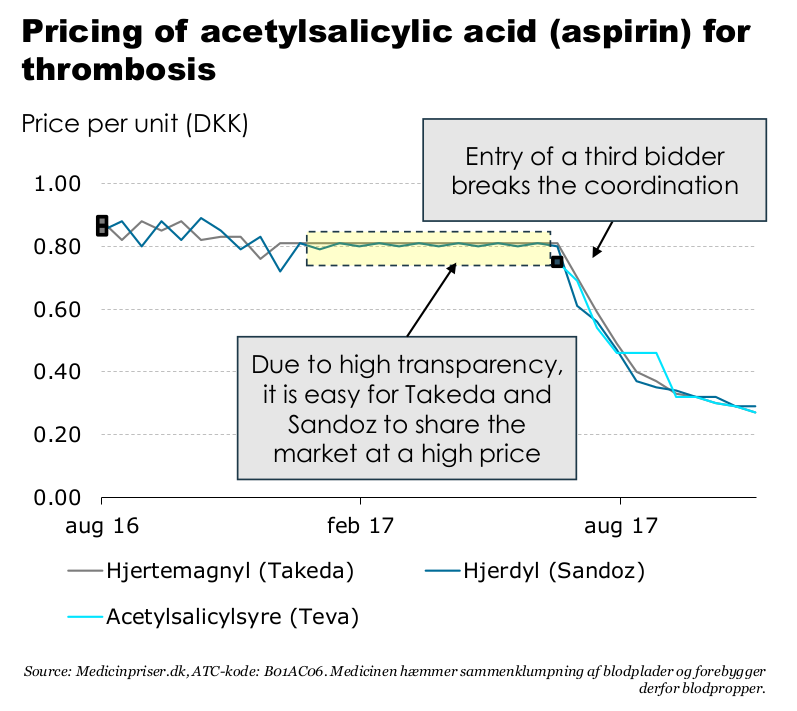
\includegraphics[width=0.6\textwidth]{figures/medprices.png}
    \caption{\textbf{Danish medicine prices} showing clear signs of tacit collusion.}
    \label{fig: medprices}
\end{SCfigure}

An example of an illegal coordination is how danish construction firms used to share bids in advance of auctions, so that companies could bid a reasonable but non-winning bid even though they didn't have the capacity to undertake the construction work. This practice was known in the industry as "keeping the customer warm", i.e. signalling that a construction company was still interested in future work, without revealing their capacity limits to the buyer. 

\subsection{Introduction to multiunit auctions}
The multiunit auctions are distinct from sequential auctions as they assume multiple units of the same item is auctioned away at once. Denote the number of units for sale $K$, each bidder submits a bid vector $b^i=(b_1^i, b_2^i, ..., b_K^i)$ which gives the willingness to pay for each item, assuming they have won all of the previous units. We can think of the bid vector as an \textit{inverse demand function}.
\\ \\
In this setting the previously studied auction formats can no longer be applied directly, instead the possible formats are 
\begin{itemize}
    \item Sealed bid discriminatory.
    (Bidders pay the sum of their winning bids)
    \item Sealed bid uniform price 
    (Bidders pay a fixed price times the number of items they win. The price is set as the clearing price which makes the demand equal supply)
    \item The Vickrey auction (also sealed)
    (Bidders pay equal to the bids they "push out" of the winning bids, note this collapses to the second price auction when $K=1$).
    \item The open bid Dutch 
    \item The open bid English 
    \item The Ausubel auction (also open)
\end{itemize}

\paragraph{Example (sealed bid)} consider the three bidders $A,B,C$ who submit bids as in figure \ref{fig: multiexample}. Each row here corresponds to a bid vector $b^A, b^B, b^C$. All of the above formats solve the problem of allocating all of the 6 units to the bidders with the highest bid, but differ in which prices are paid for each unit. 

\begin{SCfigure}[][h]
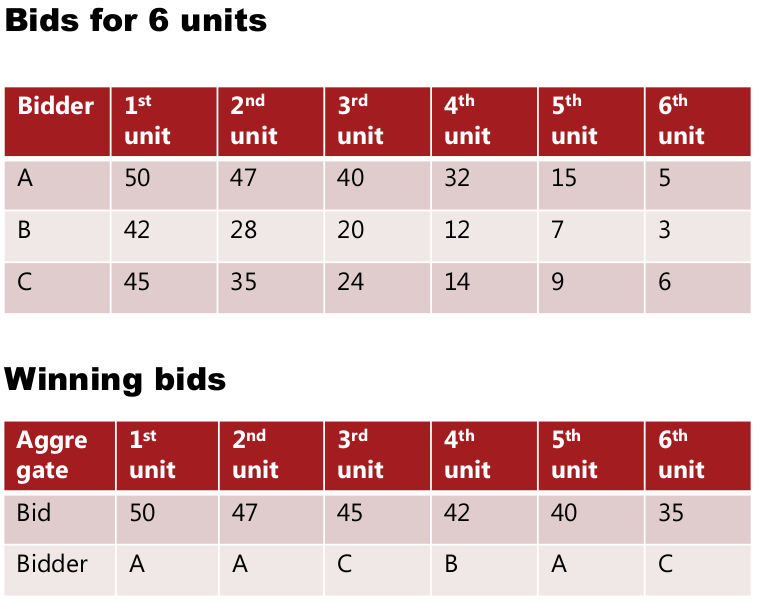
\includegraphics[width=0.6\textwidth]{figures/multibids.png}    
\caption{\textbf{Multi unit auction} example bids.}
\label{fig: multiexample}
\end{SCfigure}  

This auction will have winning bids also shown in figure \ref{fig: multiexample}. (We were shown how to calculate the prices on the blackboard).

\subsection{The day-ahead market in Northern Europe}
An example of a multiunit market is the day-ahead market for energy supply in Northern Europe. Here every hour of the following days electricity supply is auctioned away to suppliers. This is an example of a market which can produce "residual monopolies".
\\ \\
This auction is held as a uniform price auction, and so it might be benefitial to engage in demand reduction ("strategic capacity withholding"), see lecture 11.

\pagebreak
\section*{Part 2}
\section{Calculus of voting}
In this lecture we will study the equilibrium strategies in multi unit auctions. Last lecture we only saw examples of the allocation and pricing mechanisms, but not how these mechanisms influence the bidders. Consider an auction with $K$ items for sale and $N$ bidders. Each bidder draws a vector of private values 
\begin{equation}
    X^I = (X_1^i, X_2^i, ..., X_K^i)
\end{equation}
which represent the bidders marginal value of winning $k\in[1,K]$ items. Thus the total value for the bidder from winning $k$ items is $\sum_{l=1}^k X_l^k$. By assumption $X_1^i \geq X_2^i \geq ... \geq X_K^i$. These are drawn on 
\begin{equation}
    \mathcal{X} = \{x\in[0, \omega]^K: \ \forall k, x_k \geq x_{k+1} \}
\end{equation}

\paragraph{The Vickrey auction}
In the Vickrey auction the total amount paid by a bidder who wins $k^i$ units is equal to the $k^i$ largest \textit{loosing} bids of the opponents, that is 
\begin{equation}
    \sum_{k=1}^{k^i} c_{K-k^i + k}^{-i}
\end{equation}
where $c^{-i}$ is the vector of sorted highest competitor bids. We can argue to show that in Vickrey auctions it is weakly dominant to bid ones true demand vector. This is because (similar to in second price auctions) the bidder doesn't have any control of the final price paid in the Vickrey auction - it is determined by the competing bidders bids. Pretending a higher or lower demand curve either changes nothing, foregoes winning an item which would yield a positive payout or wins an item at to expensive a price. However Vickrey auctions can in some case appear unfair, because a bidder with high valuations "pushes out" weaker bidders, and thus pay a low price, while weaker bidders have to push out the strong bidder to win anything, meaning they pay high prices. 

\paragraph{Uniform value auctions}
There is no reduced form expression of the equilibrium in uniform price auctions (although outside the scope of the course it can be shown that a unique one exists with private independent values). Instead it can indirectly be shown that (Krishna p.191-192)
\begin{itemize}
    \item[1.] No bids exceeds the marginal value, that is for all elements in the value vector, bids do not exceed this value. The reason is that the bids only matter if they end up setting the price. If a bid is above the marginal value it would be costly if it ended up setting the price. 
    \item[2.] There is no shading on the first element of the bid vector. This is because the first object cannot be price setting as there is at least one item for sale, and it is the first non-winning bid that sets the price. Thus the only possible effect from shading is to risk loosing the auction. 
    \item[3.] On the remaining elements in the bid vector there is an incentive to shade ones bid, as these bids may become price-setting. This produces a tradeoff between a low price which reduces the price paid for the items one win, and a high price increasing the chance of winning another item.   
\end{itemize}

\paragraph{Discriminatory auctions}
Like the uniform case it is known that the private independent value case has an unique equilibrium, but it has no known reduced form. It is clear that there will be shading on all value as bidding ones value gives a payoff of 0. Furthermore the shading will be strongest for the first items, as it doesn't matter to the bidders if they win the first or last item. In fact it would be preferential to win the last items and let someone else buy the first items at high prices. 
\\ \\
Bidders can in some circumstances submit flat demand curves (Krishna 196-197).

\subsection{Efficiency and fairness in multiunit auctions}
Of the three covered multiunit formats only the Vickrey is generally efficient. In particular because equilibria in standard multiunit auctions are efficient iff the bidders strategies are separable and symmetric both in the objects and bidders, that is 
\begin{equation}
\forall i,k : \ \beta_k^i(x^i) = \beta(x_k^i)
\end{equation}
The uniform and discriminatory auctions does not satisfy this because the strategies depend on which item of the auction one is bidding for, i.e. the 1'st item requires a different strategy than the 3rd, so the strategies are not separable across items. 
\\ \\
As already mentioned the Vickrey auction on the other hand might be perceived as unfair in situations where bidders are not even, because the prices of the strong bidder is set by the weak bidders and oppositely. 

\section{Elections as information aggregation}
\paragraph{Revenue considerations} there is no general revenue ranking for multiunit auctions, in the sense that formats can be ranked in their expected revenue. There is however a generalized version of the revenue equivalence theorem which we will show here. The statement is that any two multiunit auctions which have the same \textit{allocation} rule will yield the same expected revenue. 
\begin{SCfigure}[][h]
    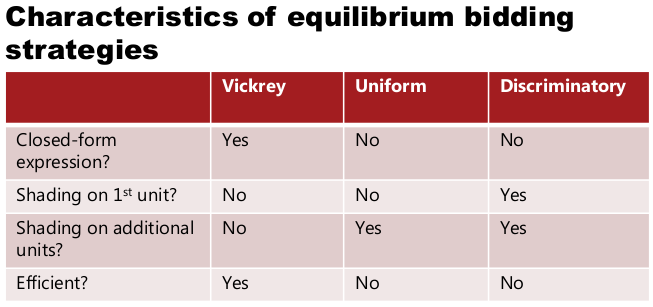
\includegraphics[width=0.6\textwidth]{figures/characteristics.png}
    \caption{\textbf{Characteristics of multiunit formats}}
\end{SCfigure}

\paragraph{Multiunit revenue equivalence}
Let $X^i=(X_1^i, X_2^i, ..., X_K^i)$ be a vector of bidder $i$'s valuations where $X_k^i$ is the marginal valuation of winning the $k$th unit. These are drawn independently from 
\begin{equation}
    \mathcal{X} = \{x \in [0,\omega]^K
    : \forall k, x_k \geq x_{k+1} 
    \}
\end{equation}
potentially with individual densities $f_i:\mathcal{X}\rightarrow [0,1]$. Now fix an auction format with a fixed equilibrium $\bm\beta=(\bm\beta^1, \bm\beta^2, ...,\bm\beta^N)$ assume that all other bidders follow the equilibrium $\bm\beta^j$. Then if bidder $i$ has value vector $\bm{x}^i$ but pretends to have values $\bm{z}^i$ and thus bids $\bm\beta^i(\bm{z}^i)$. We denote by $q_k^i(\bm{z}^i)$ the probability that bidder $i$ wins the $k$th unit, as a function of his pretended value vector. The bidders gain from pretending to have $\bm{z}^i$ can be written 
\begin{equation}
    \sum_{k=1}^K q_k^i(\bm{z}^i)x_k^i = \bm{q}^i(\bm{z}^i) \bm{x}^i
\end{equation}

By two auctions having the same allocation rule we mean exactly that the probabilities $q_k^i(\bm{z}^i)$ are the same in both auctions. Letting $m^i(\bm{z}^i)$ be the expected payment in some auction by bidder $i$ and assume that $m^i(0)=0$. The bidders expected payoff is then 
\begin{equation}
    \Pi(\bm{z}^i,\bm{x}^i) = \bm{q}^i(\bm{z}^i) \cdot \bm{x}^i - m^i(\bm{z}^i)
\end{equation}
and because in equilibrium it is optimal (by definition) to bid $\bm{\beta}^i(\bm{x}^i)$ we have 
\begin{equation}
    \forall \bm{z}^i : \ \bm{q}^i(\bm{x}^i) \cdot \bm{x}^i - m^i(\bm{x}^i) \geq \bm{q}^i(\bm{z}^i) \cdot \bm{x}^i - m^i(\bm{z}^i)
\end{equation}

(See Krishna p.205-206 for continuation, it gets quite complicated)
\\ \\
Following through with the proof it can be shown that the equilibrium payoff functions in two auctions with the same allocation rule are identical up to a constant. The additive constant arises as the payoff for a bidder with value vector $0$, so this falls out when assuming that this is 0. 

\paragraph{Example of applying multiunit revenue equivalence}
Let us consider a case with $K=3$ items for sale, and 2-unit demand from two bidders. The value vector for each bidder is IID $X^i=(X_1^i, X_2^i)$ on $[0,1]^2$, and naturally $X_1^i>X_2^i$. We know that in the Vickrey format it is optimal to submit truthful bids, so 
\begin{equation}
    (b_1^i, b_2^i) = (x_1^i, x_2^i)
\end{equation}
because both bidders have two unit demand, they face competing bids 
\begin{equation}
    c^{-i}  = (x_1^j, x_2^j, 0)
\end{equation}
Both bidders are guaranteed to win one unit, as there are three for sale and each bidder only wants two. One bidder will therefore win two items and pay $x_2^j + 0$, while the other bidder wins one item at a price of $0$. For some given $x_1, x_2$ the expected payment is thus 
\begin{equation}
    m^V(\bm{x}) = P(X_2 < x_2)\cdot E[X_2 | X_2 < x_2] = \int_0^{x_2} y f_2(y) \ dy
\end{equation}
i.e. the other bidders expected bid on the second unit (independence implies we can drop the superscripts), given it is smaller than $x_2$, times the probability this happens. 
\\ \\
Now consider the equivalent uniform auction. We know that the bids here will be $(b_1^i, b_2^i) = (x_1^i, \beta(x_2^i))$. Assuming such a $\beta$ exists and it is increasing we can see that the uniform auction will be efficient. This is in essence because both bidders will certainly win 1 unit, and only win a second if $b_2^i > b_2^j$ implying by monotonicity $x_2^i > x_2^j$. Knowing this the expected payment for bidder $i$ in a uniform auction must be the sum of 1) the expected payment when winning two units, at a price of $x_2^j$ (the highest non-winning bid) and 2) the expected payment when winning one item, which is bidder $i$'s own bid for the second item (the highest non-winning bid) times the probability of this happening, that is 
\begin{equation}
    m^U(\bm{x}) = \int_0^{x_2} 2 \beta(y)f_2(y) \ dy 
    + (1- F_2(x_2)) \beta(x_2)
\end{equation}
Now due to the revenue equivalence theorem (applicable because we have argued that both auctions are efficient) it must be that $\forall z\in[0, \omega]: \ m^V(x_1, z)=m^U(x_1, z)$, i.e.
\begin{equation}
    \int_0^{z} y f_2(y) \ dy = 
    \int_0^{z} 2 \beta(y)f_2(y) \ dy 
    + (1- F_2(z)) \beta(z)   
\end{equation}
Taking the derivative w.r.t $z$ gives 
\begin{equation}
    \begin{split}
    z f_2(z) &= 2 \beta(z) f_2(z) + (1-F_2(z)) \beta'(z) - f_2(z)\beta(z)  \\ 
    &=\beta(z) f_2(z) + (1-F_2(z)) \beta'(z)
    \end{split} 
\end{equation}
Using that $\beta(0)=0$ this can be written as 
\begin{equation}
    \beta'(z) = (z-\beta(z)) \lambda_2(z), \quad \lambda_2(z) \equiv \frac{f_2(z)}{1- F_2(z)}
\end{equation}
Solving this differential equation gives 
\begin{equation}
    \beta(z) = \int_0^z y \lambda_2(y) \ dL(y|z)
\end{equation}
where $L(y|z)=\exp \left(- \int_y^z   \lambda_2(t) \ dt \right)$ which is identical to the integrating factor also used in the single-item auction. Thus we have been able to derive the closed form equilibrium strategy in this very particular case of uniform pricing. 

\paragraph{Discriminatory auction} 
A similar argument for efficiency can be made in the discriminatory price auction, once again on the grounds that in fact only one item is truely "for sale" as bidders only want two each, meaning they get one item free each. Arguing that the demand will be flat in this case and going through the calculations of equating expected payments it can be shown that in this case the bid for both the first and second unit will follow 
\begin{equation}
    \beta(x_2) = \frac{1}{1 + F_2(x_2)} \int_0^{x_2} y f_2(y) \ dy
\end{equation}
which notably does not at all depend on the value of $x_1$.

\pagebreak
\section{Lecture 21 - Competence vs. representation}
In this lecture we study the problem of selecting politicians who at the same time represent a voters preferred policies and carry the competencies to get these policies implemented. In the two extreme cases we might have either 
\begin{itemize}
    \item[1.] All politicians are equally competent, but voters disagree on the optimal policy.
    \item[2.] All voters(/politicians) agree on what is the optimal policy but politicians vary in their competence.
\end{itemize}
When considering some mix of these two extremes a tradeoff arises between competence and policy. In particular all voters wants to be represented by someone competent, but differ what policy attitudes they prefer.

\subsection{Model by \cite{mattozzi_right_2018}}
The model is very similar to the regular downsian model. A continuum of citizens with measure 1 vary in their income and are taxed with some rate $\tau$ to provide a public good. Candidates for elections are drawn from the population and have no commitment to their proposals after election. 

Voters are assumed to live in one of $2n +1$ districts, each of which elect a single legislator. The level of $g$ is set independently for each district, but the tax rate is fixed at a single value, so legislators goal is to bargain a high level of expenditures in their own district.

\paragraph{Voters} 
Voters are split in two groups, the "poor/unsuccessful" with income $y_l$ and the "rich/sucessful" with income $y_h = \eta y_l$. Some share $\gamma>1/2$ of voters are poor. 
The voters utility is quasi-linear in preferences over after-tax income and the level of public good provided in their district. I.e.
\begin{equation}
    u_{ij} =(1-\tau) y^i + g(\pi^j \tau \bar{y})
\end{equation}
where $\bar{y}$ is the average income across all voters and $\pi^j$ is the proportion of total revenue $\tau \bar{y}$ that goes to district $j$. From this we see that given any split $\pi^j$ low type citizens prefer a higher tax rate than high type citizens\footnote{See $\partial_{\tau} u_{ij}=-y^i + \pi^j \bar{y} g'(\pi^j \tau \bar{y})$. Thus in optimum 
\begin{equation}
    \tau = \frac{1}{\pi^j \bar{y}} g'^{-1}(\frac{y^i}{\pi^j \bar{y}})
\end{equation}}
Letting $\tau_l^*$ and $\tau_h^*$ denote the preferred tax rates when revenue is split equally between the districts it must be that $\tau_l^* > \tau_h^*$. 

Obviously given a $\tau$ the voters in district $j$ prefers $\pi^j$ to be set as high as possible.

\paragraph{Elections}
Elections are held at the same time across all districts. In each election one low type voter and one high type voter runs, and we assume that voters are distributed such that $\lambda>1/2$ of districts have a majority of low type candidates. Applying the median voter theorem, any district with a majority of poor individual will have a median voter who is also poor who decides the election, and any rich district will have a rich median voter who decides the election.

\paragraph{Legislature}
The legislature might either be majority rich or majority poor depending on the elections. The way legislature works is that they first vote on a tax rate $\tau$ and then bargain for the shares $\pi^j$ that goes to each district.
\\ \\ 
In the bargaining phase we assume that high income individuals are better at bargaining, by the reasoning that if you do well in the private sector you will also do well in the legislature. The abilities of legislators $(a_1, a_2,...,a_N)$ are set such that $a_l=1$ and $a_h = \eta$. The parameter $\gamma$ governs how much ability matters for bargaining, and so the outcome of bargaining is $\pi^{j*}(a_1,a_2,...,a_N|\gamma)$. Now if bargaining ability has no influence the outcome for each district will be $\pi^{j*}(a_1, ...,a_N|\gamma = 0)\rightarrow1/N$, that is districts simply split the revenue equally. We will further assume that $\partial_{a_j} \pi^{j*}\geq 0$ and $\partial_{a_k} \pi^{j*} \leq 0$ for all $j\neq k$. This simply says that higher bargaining ability of the legislator from district $j$ increases the spending in district $j$ won in bargaining, while higher bargaining abilities of legislators from other districts decrease the spending in district $j$.
\\ \\
The core question in this model is then who voters will elect, someone who share their views on the optimal $\tau$ or someone who can bargain a large share of the tax revenue to the home district. Naturally high type voters prefer to vote for a high type candidate, as they can get both low taxes and competent bargaining from the same candidate. Low income voters however face a tradeoff between getting a legislator who votes for higher taxes and one who bargains well. How this plays out depends on the value of $\gamma$:
\begin{itemize}
    \item[1.] if $\gamma = 0$ there os no tradeoff, so poor districts elect poor candidates. Since there is a majority of poor candidates the legislature will be majority poor and select a tax of $\tau_l^*$. This is a fully representative equilibrium as the median voter is low, so is the median legislator and the outcome is in accordance with their preferences.
    \item[2.] if $\gamma$ is sufficiently high, voters concern with electing a competent politician dominates, so all districts select a high type candidate and the legislature implements $\tau_h^*$. In this equilibrium there is no representativeness, as no legislators will be low type even though a majority of voters are. 
    \item[3.] if $\gamma$ is moderate once a majority $n+1$ have elected a low type it is certain that a low type candidate will by the MVT set the tax rate, and the remaining poor districts become free to select a candidate with high bargaining abilities meaning $n$ high type candidates will enter the legislature. In this case the equilibrium is somewhat representative, as the tax rate is set by a low type, but there is a over representation of high type legislators in the legislature and as a consequence the tax rate will be set lower than $\tau_l^*$ in anticipation of bargaining, in which the districts with low type legislators will have to fund some of the high-type districts spending. 
\end{itemize} 

In summary this model predicts a tradeoff between electing competent politicians and getting a high tax rate for low-income individuals in district voting systems. 

\subsection{Empirics \citep{dal_bo_who_2017}}
Using purely descriptive analysis \cite{dal_bo_who_2017} use a dataset with the entire swedish population as well as various special information on politicians and candidates for elections.

This includes information from conscription tests including IQ and in some cases "leadership tests" undertaken with a psychologist.

To not mechanically measure a correlation between being in the "elite" (a politician) and competence they use parents background as a proxy for representation - i.e. if ones parents were regular people, it is fair to assume that one represents this group, and not the "elite" in the legislature (?). 


\begin{SCfigure}[][h]
    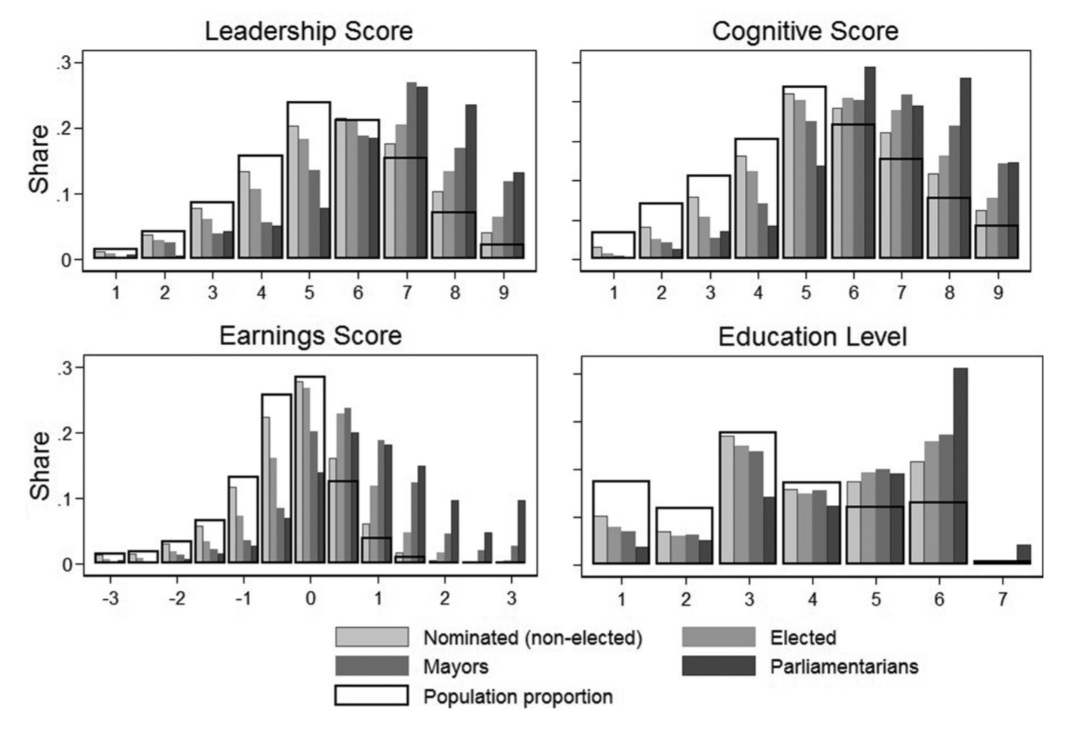
\includegraphics[width=0.6\textwidth]{figures/dal_bo_1.png}
    \caption{\textbf{Results from \cite{dal_bo_who_2017}} The results compares the distribution of various measures of competence with the population distribution of these traits.}    
\end{SCfigure}

The authors find a systematic tendency for politicians to be high competence individuals, with this trend being stronger the higher the office held. This selection is much less pronounced when comparing to parents background. In the sense that the relevant dimension for measuring representation is across generations this suggests that representation issues are not nearly as large as they could have been. In particular it seems that all parties select candidates who themselves are high competence, but tend to favor candidates whose parental background lies in different parts of the income distribution. 

Importantly the lack of relation between parents background and being a politician does not mean that there is no intergenerational persistence in income and abilities etc. Instead the parties have stronger selection for candidates with background lower in the income distribution, evening out the correlation. In other words if your parents are rich you dont have to be very clever to become a politician, but if they're poor you need to be very smart. This selection removes the apparent relation between parents abilities and being a politician.
\\ \\
In summary in Sweden politicians are highly competent compared to the population, but are representative in terms of their background.
%=================
\newpage
% CHANGE THIS IF YUOR BIBFILE HAS A DIFFERENT NAME
\bibliography{references.bib}

\end{document}
